\chapter{FreeRTOS functional safety additions}
\label{freertos_modification}

\section{Timed tasks addition}

\subsection{Introduction}

Atop of all FreeRTOS functionality ability of measuring task's run time and its total time (running + other states) is not provided. Such feature is extremely useful for hard real-time embedded systems. In such systems breaching the deadline means failure of the system.

Adding the aforementioned timers to the tasks means ability to detect if the task ran for too long or it didn't get enough processor time. When such event has occurred it can be properly handled. For example, for an embedded system that is periodically polling a speed of rotation of an engine if it isn't polled in time it can raise an alarm to force the reading.

\subsection{Architecture}


When timed tasks are created two software timers are created tied to it. One is called overrun timer and is used to detect when the task is in a running state longer than defined. Second, overflow timer is used to detect if the task is running properly asynchronously i.e. timer doesn't stop ticking even if the timed task is inactive.  

The overflow timer is started when the timed task is switched into the first time. It is started from the context switch. Code section is shown in \autoref{fig:freertos_overflow_start}. Function prvStartOverflowTimer checks if the timer is started and if it isn't it starts the timer otherwise it doesn't do anything.


\begin{figure}[H]

      \centering
      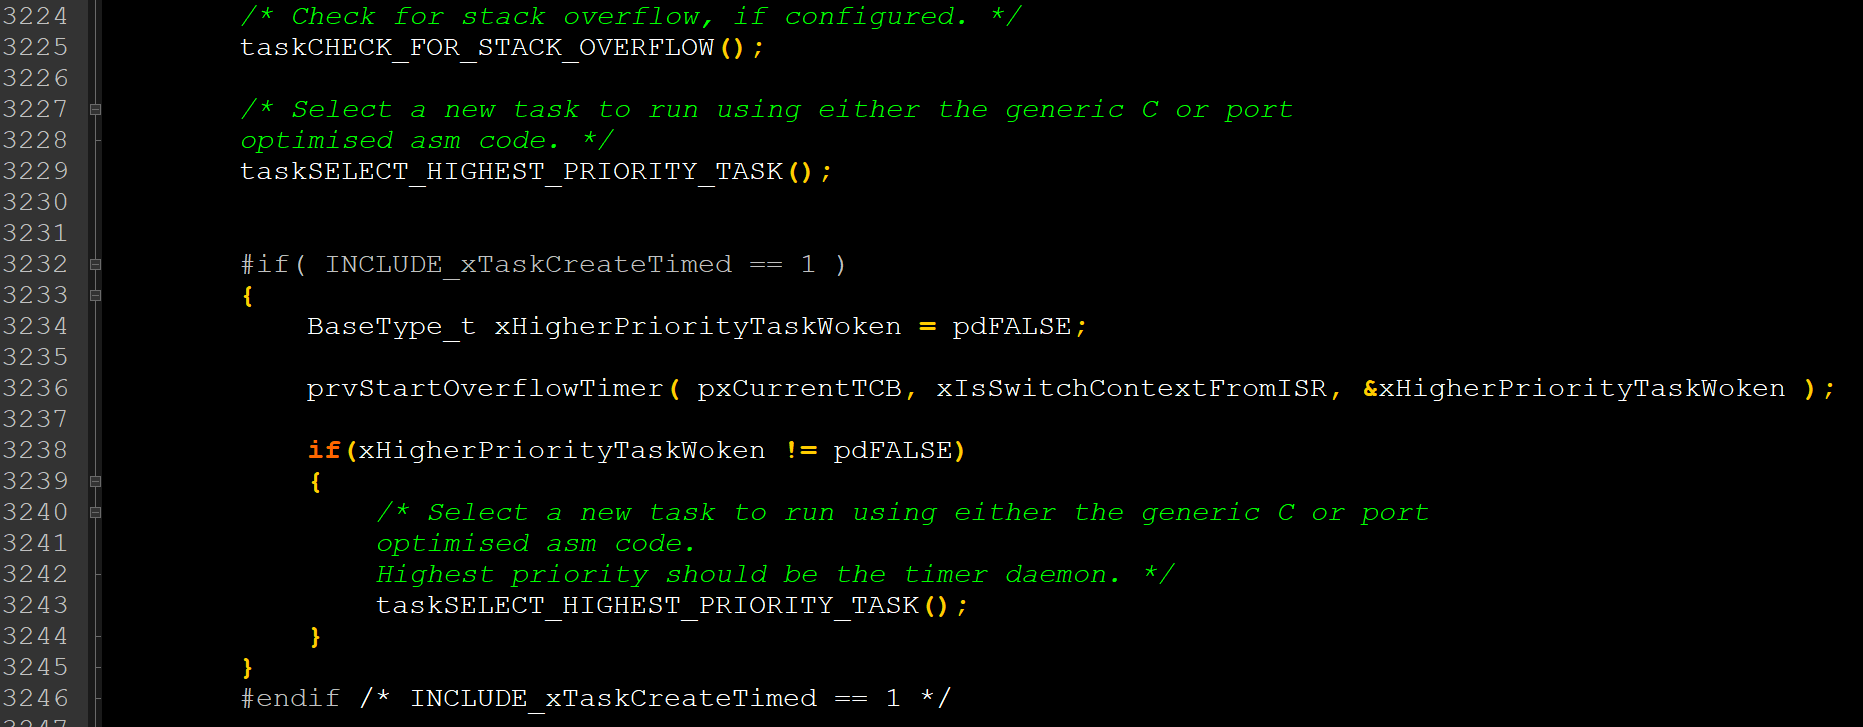
\includegraphics[width=\linewidth]{images/freertos_overflow_start.png}
      \caption{Starting of the overflow timer from the file task.c}
      \label{fig:freertos_overflow_start}
    
\end{figure}

The overrun timer is, in the beginning, just a TickType\textunderscore t variable xOverrunTicks in the task's control block. It is incremented every tick timed task is running. When it is over the maximal value it start a software timer with a timeout of 1 tick. Timer daemon triggers the overrrun callback one tick later. Code for incrementing (\autoref{fig:freertos_overrun_increment}) is called from the function xTaskIncrementTick which itself is called from the tick interrupt. Overrun timer (of period 1 tick) is started from the context switch function, with code shown in \autoref{fig:freertos_overrun_start}.

\begin{figure}[H]

      \centering
      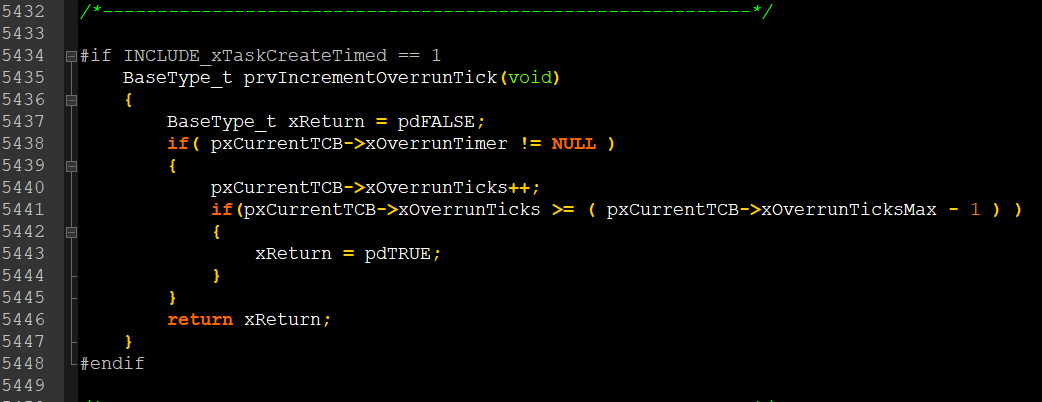
\includegraphics[width=\linewidth]{images/freertos_overrrun_increment.png}
      \caption{Incrementing of the overrun timer from the file task.c}
      \label{fig:freertos_overrun_increment}
    
\end{figure}

\begin{figure}[H]

      \centering
      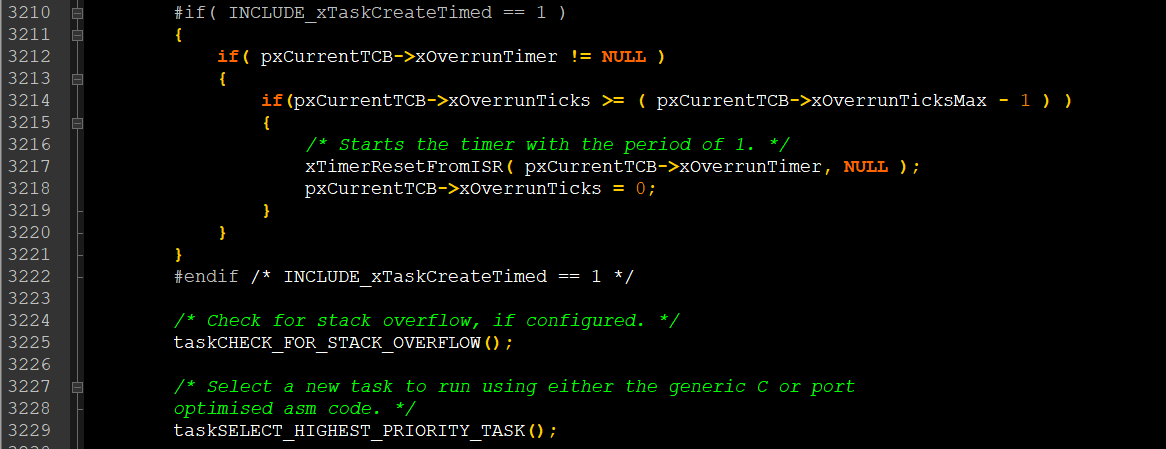
\includegraphics[width=\linewidth]{images/freertos_overrun_start.png}
      \caption{Starting of the overrun timer from the file task.c}
      \label{fig:freertos_overrun_start}
    
\end{figure}


 Next three figures showcase how the timed tasks work. \autoref{fig:timed_example_overrun} shows when is overrun timer triggered. Similarly, \autoref{fig:timed_example_overflow} showcases how the overflow timer works. Finally, \autoref{fig:timed_example_reset} shows how reseting the timed task suppresses the timeout of overflow and overrun timers.

\begin{figure}[H]

      \centering
      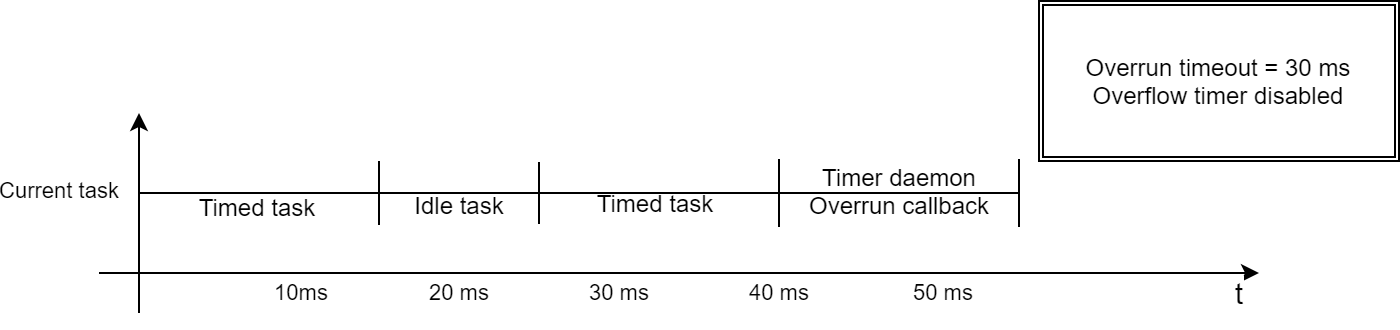
\includegraphics[width=\linewidth]{images/timed_example_overrun.png}
      \caption{Timed task with overrun timeout of 30 ms}
      \label{fig:timed_example_overrun}
    
\end{figure}

\begin{figure}[H]

      \centering
      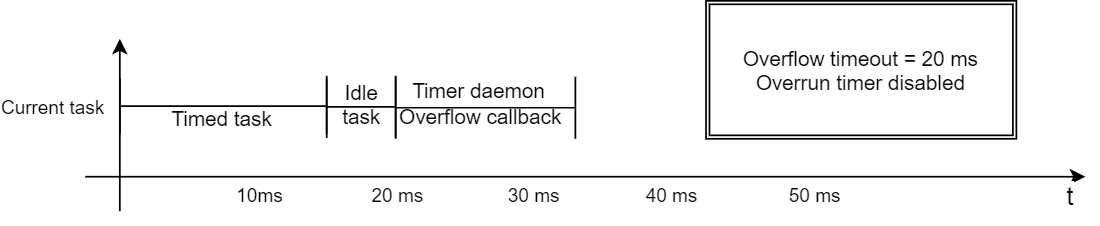
\includegraphics[width=\linewidth]{images/timed_example_overflow.png}
      \caption{Timed task with overflow timeout of 20 ms}
      \label{fig:timed_example_overflow}
    
\end{figure}

\begin{figure}[H]

      \centering
      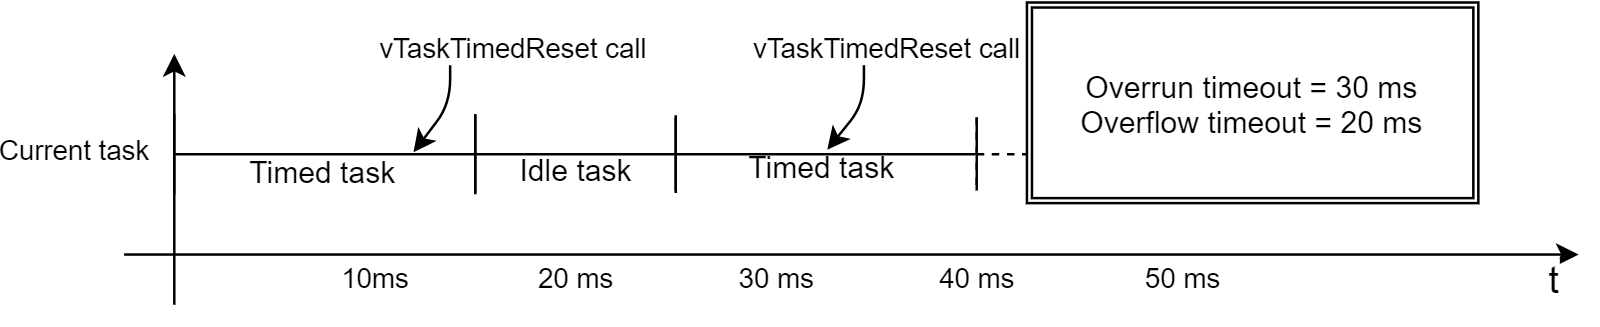
\includegraphics[width=\linewidth]{images/timed_example_reset.png}
      \caption{Timed task with both timers that resets in time}
      \label{fig:timed_example_reset}
    
\end{figure}

vTaskDelete function is changed so that deleting tasks also deletes their timers.

\subsection{Limitiations}

Static create of the function is not available.

Timer callback functions are called by the timer daemon and its priority determines when the callback will be called. It is recommended that timer deamon has the highest priority.

\section{Replicated tasks}

\subsection{Introduction}

Redundancy is a common term with safety hardware, but the redundancy can be achieved with the software. As is demonstrated with the replicated tasks. As the name suggests, when replicated tasks are created they make more parallel instances and they compare outputs of each other to assure no errors happened. 

Hardware redundancy has the advantage of detecting the fault as early as possible at the cost of increased hardware. On the other hand, software redundancy is useful when the system cost is the restriction ss no additional hardware is needed. 

\noindent Two types of replicated tasks are implemented:
\begin{itemize}
    \item 2oo2\footnote{MooN is read as M out of N. It shows how many valid outputs have to be present for valid operation e.g. 1oo2 means 1 valid output out of 2 have to be present for a valid operation} configuration or without recovery
    \item 2oo3 configuration or with recovery
\end{itemize}

Recovery of 2oo3 configuration can be achieved with voting logic. Voting logic can determine which two tasks have the same output and make it a valid one. Same is not possible with 2oo2 voting logic.


\subsection{Architecture}

Replicated tasks have an ability to detect errors using at least two tasks performing identical operations. Tasks are independently processed by the processor. Output variables from tasks are compared in real time. In case of discrepancy in the output variables, an error callback is called where user can process the error.

\autoref{fig:replicated_example} shows how replicated task with recovery works. It shows that all instances wait on the barrier. When all tasks have arrived their compare values are compared. In case of an missmatch, the callback given on task creation is called. 


\begin{figure}[H]

      \centering
      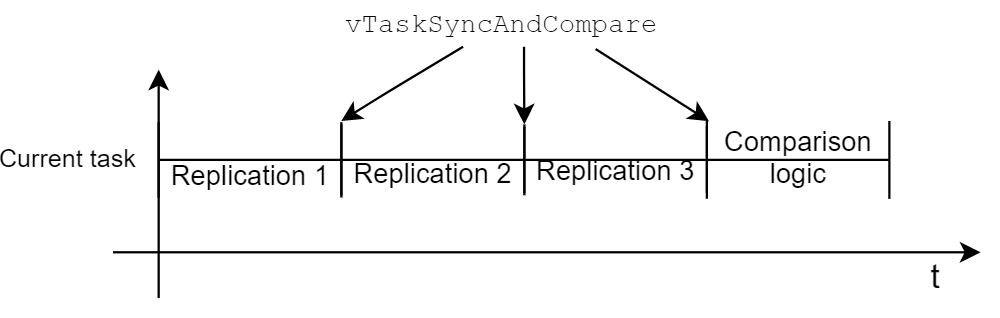
\includegraphics[width=\linewidth]{images/replicated_example.png}
      \caption{Replicated task with redundancy}
      \label{fig:replicated_example}
    
\end{figure}

Comparison logic is not a new task for itself. It is done within one of the tasks. Whichever arrives last. vTaskDelete function was modified so that when one of the replicated sub-tasks delete is requested all linked will be deleted. Tasks are linked over the TCBs\footnote{TCB - Task control block}.

\subsection{Limitiations}

Static create of the timed tasks is not available.

\section{Command reference}

Timed tasks:
\begin{itemize}

    \item \nameref{rt_cmd:xTaskCreateTimed}
    \item \nameref{rt_cmd:vTaskTimedReset}
    \item \nameref{rt_cmd:xTimerGetTaskHandle}
    
\end{itemize}

\noindent Replicated tasks:
\begin{itemize}

    \item \nameref{rt_cmd:xTaskCreateReplicated}
    \item \nameref{rt_cmd:xTaskSetCompareValue}
    \item \nameref{rt_cmd:vTaskSyncAndCompare}
    
\end{itemize}

\noindent General added functions:
\begin{itemize}

    \item \nameref{rt_cmd:eTaskGetType}
    \item \nameref{rt_cmd:xTimerPause}
    \item \nameref{rt_cmd:xTimerPauseFromISR}
    \item \nameref{rt_cmd:xTimerResume}
    \item \nameref{rt_cmd:xTimerResumeFromISR}
    \item \nameref{rt_cmd:xTimerIsTimerActiveFromISR}
    
\end{itemize}

\subsection{xTaskCreateTimed -  Creates a timed task.}
\label{rt_cmd:xTaskCreateTimed}

\begin{minted}[breaklines, linenos]{c}

BaseType_t xTaskCreateTimed( TaskFunction_t pxTaskCode,
                    const char * const pcName,
                    const configSTACK_DEPTH_TYPE usStackDepth,
                    void * const pvParameters,
                    UBaseType_t uxPriority,
                    TaskHandle_t * const pxCreatedTask,
                    TickType_t xOverrunTime,
                    WorstTimeTimerCb_t pxOverrunTimerCb,
                    TickType_t xOverflowTime,
                    WorstTimeTimerCb_t pxOverflowTimerCb )
            
\end{minted}

\begin{lstlisting}        
Create a new timed task and add it to the list of tasks that are ready to
run.

Overrun timer is synchronous with the task and its counter is incremented
only when timed task is in running state. Overrun callback is called from
timer daemon. When timed task overruns it sends a signal to the timer daemon
and when callback is called is dependent on daemon's priority. If overrun
timer is not used send 0 for xOverrunTime or NULL for the callback.

Overflow timer is asynchronous with the task and its counter is incremented
every tick regardless of the state. Callback is called from timer daemon and
its punctuality is dependent on timer daemon's priority. If overflow timer
is not used send 0 for xOverflowTime or NULL for the callback.

Internally, within the FreeRTOS implementation, tasks use two blocks of
memory.  The first block is used to hold the task's data structures.  The
second block is used by the task as its stack.  If a task is created using
xTaskCreateTimed() then both blocks of memory are automatically dynamically
allocated inside the xTaskCreate() function.  (see
http://www.freertos.org/a00111.html). Static version of the function is not
implemented.

Input paramters:
 - pvTaskCode - Pointer to the task entry function.  Tasks
must be implemented to never return (i.e. continuous loop).

- pcName - A descriptive name for the task.  This is mainly used to
facilitate debugging.  Max length defined by configMAX_TASK_NAME_LEN - default is 16.

- usStackDepth -The size of the task stack specified as the number of
variables the stack can hold - not the number of bytes.  For example, if
the stack is 16 bits wide and usStackDepth is defined as 100, 200 bytes
will be allocated for stack storage.

- pvParameters - Pointer that will be used as the parameter for the task
being created.

- uxPriority - The priority at which the task should run.  Systems that
include MPU support can optionally create tasks in a privileged (system)
mode by setting bit portPRIVILEGE_BIT of the priority parameter.  For
example, to create a privileged task at priority 2 the uxPriority parameter
should be set to ( 2 | portPRIVILEGE_BIT ).

- pvCreatedTask - Used to pass back a handle by which the created task
can be referenced.

- xOverrunTime - Runtime of the task after which callback will be called.

- pxOverrunTimerCb - Pointer to the function that will be called if task
runs longer than xOverrunTime without reseting the timed task. Overrun timer
is synchronous with the task and its tick is only incremented when timed
task is in running state.

- xOverflowTime - Asynchronous timer time. After xOverflowTime
pxOverflowTimerCb will be called.

- pxOverflowTimerCb - Pointer to the function that will be called after
xOverflowTime. Overflow timer is asynchronous from the task and its value is
incremented every tick.

Returns pdPASS if the task was successfully created and added to a ready
list, otherwise an error code defined in the file projdefs.h
Example usage:

\end{lstlisting}

\begin{minted}[breaklines, linenos]{c}
 // Task to be created.
 void vTaskTimedCode( void * pvParameters )
 {
     for( ;; )
     {
         // Task code goes here.

         // Reset the timer.
         vTaskTimedReset(NULL);
     }
 }

// Function to be called if timer overflows.
void vTaskOverflowCallback ( WorstTimeTimerHandle_t xTimer )
{
    // Timeout callback code.

    // Maybe task deletion is needed. Calling vTaskDelete automatically deletes
    // the timer too. Do NOT delete the timer directly. That will cause
    // undefined behavior when deleting the task.
    vTaskDelete( xTimerGetTaskHandle( xTimer ) );
}
// Function to be called if timer overflows.
void vTaskOverrunCallback ( WorstTimeTimerHandle_t xTimer )
{

    // Timeout callback code.

    // Maybe task deletion is needed. Calling vTaskDelete automatically deletes
    // the timer too. Do NOT delete the timer directly. That will cause
    // undefined behavior when deleting the task.
    vTaskDelete( xTimerGetTaskHandle( xTimer ) );
}

 // Function that creates a task.
 void vOtherFunction( void )
 {
 static uint8_t ucParameterToPass;
 TaskHandle_t xHandle = NULL;

     // Create the task, storing the handle.  Note that the passed parameter ucParameterToPass
     // must exist for the lifetime of the task, so in this case is declared static.  If it was just an
     // an automatic stack variable it might no longer exist, or at least have been corrupted, by the time
     // the new task attempts to access it.
     xTaskCreate( vTaskCode,
                  "NAME",
                  STACK_SIZE,
                  &ucParameterToPass,
                  tskIDLE_PRIORITY,
                  &xHandle,
                  pdMS_TO_TICKS(1 * 1000),
                  vTaskOverrunCallback,
                  pdMS_TO_TICKS(2 * 1000),
                  vTaskOverflowCallback );
     configASSERT( xHandle );

     // Use the handle to delete the task.
     if( xHandle != NULL )
     {
         vTaskDelete( xHandle );
     }
 }

\end{minted}

\subsection{vTaskTimedReset -  Resets the timer of timed task.}
\label{rt_cmd:vTaskTimedReset}


\begin{minted}[breaklines, linenos]{c}
void vTaskTimedReset( TaskHandle_t pxTaskHandle )
\end{minted}

\begin{lstlisting}
Reset the timer of the timed task.

- Warning - Shall only be used for timed tasks.

Input parameters:

- pxTaskHandle - Handle of the task whose timer shall be reset.
Passing a NULL handle results in reseting the timer of the calling task.

Example usage:
\end{lstlisting}

\begin{minted}[breaklines, linenos]{c}
void vTimedTask( void * pvParameters )
{
    for( ;; )
    {
        // Task code goes here.

        vTaskTimedReset(NULL);
    }
}
\end{minted}

\subsection{xTimerGetTaskHandle -  Gets the corresponding timed task handle from the timer handle.}
\label{rt_cmd:xTimerGetTaskHandle}
\begin{minted}[breaklines, linenos]{c}
TaskHandle_t xTimerGetTaskHandle( const TimerHandle_t xTimer )
\end{minted}
\begin{lstlisting}
Returns the timed task handle assigned to the timer. Task handle is an union
with timer ID and that is why they are mutually exclusive.

Task handle is assigned to the timer when creating the timed task.

WARNING: Setting the timer ID also sets the task handle. Changing the timer
ID can lead to undefined behavior.

Input parameters:

- xTimer - The timer being queried.

Example usage:

- See xTaskCreateTimed

\end{lstlisting}
\subsection{xTaskCreateReplicated -  Creates a replicated task.}
\label{rt_cmd:xTaskCreateReplicated}

\begin{minted}[breaklines, linenos]{c}
BaseType_t xTaskCreateReplicated( TaskFunction_t pxTaskCode,
                                  const char * const pcName,
                                  const configSTACK_DEPTH_TYPE usStackDepth,
                                  void * const pvParameters,
                                  UBaseType_t uxPriority,
                                  TaskHandle_t * const pxCreatedTask,
                                  uint8_t ucReplicatedType,
                                  RedundantValueErrorCb_t pxRedundantValueErrorCb )
\end{minted}

\begin{lstlisting}
Create a new replicated task and add it to the list of tasks that are ready
to run. Replicated task is used to achieve redundancy of the software at the
expense of slower execution. Task executes slower because it is replicated
two or three times. Depending  on the type chosen. On every call to
vTaskSyncAndCompare task is suspended until every replicated task arrives to
the same point. When every task is in the synchronization function
comparison is done. If any of the comparison results differ callback
function pxRedundantValueErrorCb is called. In the callback function
user can access the compare values and choose whether to delete all the
tasks.

Internally, within the FreeRTOS implementation, tasks use two blocks of
memory.  The first block is used to hold the task's data structures.  The
second block is used by the task as its stack.  If a task is created using
xTaskCreateReplicated() then both blocks of memory are automatically
dynamically allocated inside the xTaskCreateReplicated() function.  (see
http://www.freertos.org/a00111.html). Static version of this function is not
implemented.

Input parameters:
- pvTaskCode - Pointer to the task entry function.  Tasks
must be implemented to never return (i.e. continuous loop).

- pcName - A descriptive name for the task.  This is mainly used to
 facilitate debugging.  Max length defined by configMAX_TASK_NAME_LEN - default
 is 16.

- usStackDepth - The size of the task stack specified as the number of
variables the stack can hold - not the number of bytes.  For example, if
the stack is 16 bits wide and usStackDepth is defined as 100, 200 bytes
will be allocated for stack storage.

- pvParameters - Pointer that will be used as the parameter for the task
being created.

- uxPriority - The priority at which the task should run.  Systems that
include MPU support can optionally create tasks in a privileged (system)
mode by setting bit portPRIVILEGE_BIT of the priority parameter.  For
example, to create a privileged task at priority 2 the uxPriority parameter
should be set to ( 2 | portPRIVILEGE_BIT ).

- pvCreatedTask - Used to pass back a handle by which the created task
can be referenced.

- ucReplicatedType - Valid values: taskREPLICATED_NO_RECOVERY and
taskREPLICATED_RECOVERY. No recovery is faster as it created only two
instances, but recovery is not possible. Recovery creates three identical
tasks. Recovery is possible with 2 out of 3 logic.

- pxRedundantValueErrorCb - Function to be called when compare values do
not match. Return value determines whether calling redundant task will be
deleted.

Returns pdPASS if the task was successfully created and added to a ready
list, otherwise an error code defined in the file projdefs.h


Example usage:
\end{lstlisting}
\begin{minted}[breaklines, linenos]{c}
// Task to be created.
void vTaskCode( void * pvParameters )
{
    for( ;; )
    {
        // Task code goes here.

        vTaskSyncAndCompare(&xCompareValue);
    }
}

// NOTE: This function is called from the redundant task and not daemon.
uint8_t ucCompareErrorCb (CompareValue_t * pxCompareValues, uint8_t ucLen)
{
    // Iterate through compare values.
    for(uint8_t iii = 0; iii < ucLen; i++)
    {
        pxCompareValue[iii]
        .
        .
        .
    }

    return pdTRUE; // Signaling to delete the redundant task.
}

// Function that creates a task.
void vOtherFunction( void )
{
static uint8_t ucParameterToPass;
TaskHandle_t xHandle = NULL;

    // Create the task, storing the handle.  Note that the passed parameter ucParameterToPass
    // must exist for the lifetime of the task, so in this case is declared static.  If it was just an
    // an automatic stack variable it might no longer exist, or at least have been corrupted, by the time
    // the new task attempts to access it.
    xTaskCreateReplicated( vTaskCode, "NAME", STACK_SIZE, &ucParameterToPass, tskIDLE_PRIORITY, &xHandle, taskREPLICATED_RECOVERY, ucCompareErrorCb );
    configASSERT( xHandle );

    // Use the handle to delete the task.
    if( xHandle != NULL )
    {
        vTaskDelete( xHandle );
    }
}

\end{minted}

\subsection{xTaskSetCompareValue -  Sets a compare value for the calling task.}
\label{rt_cmd:xTaskSetCompareValue}

\begin{minted}[breaklines, linenos]{c}
void xTaskSetCompareValue( CompareValue_t xNewCompareValue )

\end{minted}
\begin{lstlisting}
Sets the compare value. Compare value is used with replicated tasks. They
are used in vTaskSyncAndCompare function for figuring if there is a
difference between the tied task executions.
Input parameters:
- xNewCompareValue - New compare value to set.

\end{lstlisting}
\subsection{vTaskSyncAndCompare -  Syncronizes the replicated tasks and compares compare values.}
\label{rt_cmd:vTaskSyncAndCompare}

\begin{minted}[breaklines, linenos]{c}
void vTaskSyncAndCompare( const CompareValue_t * const pxNewCompareValue )


\end{minted}
\begin{lstlisting}
Waits until every replicated task is finished. When every task is finished
function compares the compare values and if there is a mismatch it calls the
predefined callback.

- Warning - Shall only be used for replicated tasks.

Input parameters:

- pxNewCompareValue - Pointer of the compare value to be copied from. If
NULL is passed in, previous compare value is used.

Example usage:
\end{lstlisting}
\begin{minted}[breaklines, linenos]{c}
void vReplicatedTask( void * pvParameters )
{
    for( ;; )
    {
        // Task code goes here.

        vTaskSyncAndCompare(&xCompareValue);
    }
}

\end{minted}

\subsection{eTaskGetType -  Get the type of the task.}
\label{rt_cmd:eTaskGetType}
\begin{minted}[breaklines, linenos]{c}
eTaskType eTaskGetType( TaskHandle_t pxTaskHandle )
\end{minted}
\begin{lstlisting}
Get the type of the task.

Input parameters:

- pxTaskHandle - Handle of the task to be queried.  Passing a NULL
handle results in getting the type of calling task.

\end{lstlisting}

\subsection{xTimerPause -  Pauses the timer.}
\label{rt_cmd:xTimerPause}

\begin{minted}[breaklines, linenos]{c}
BaseType_t xTimerPause( TimerHandle_t xTimer, TickType_t xTicksToWait )
\end{minted}

\begin{lstlisting}
Timer functionality is provided by a timer service/daemon task.  Many of the
public FreeRTOS timer API functions send commands to the timer service task
through a queue called the timer command queue.  The timer command queue is
private to the kernel itself and is not directly accessible to application
code.  The length of the timer command queue is set by the
configTIMER_QUEUE_LENGTH configuration constant.

xTimerPause() pauses a timer. If timer was not running before it is ignored.
Pausing remembers how many ticks until the deadline are needed and on next
xTimerResume() timer will trigger only after the ticks set by pause.

Pausing assures timer is in stopped state.
 
- xTimer - The handle of the timer being paused.

- TicksToWait - Specifies the time, in ticks, that the calling task should
be held in the Blocked state to wait for the stop command to be successfully
sent to the timer command queue, should the queue already be full when
xTimerPause() was called.  xTicksToWait is ignored if xTimerPause() is called
before the scheduler is started.

Returns pdFAIL if the pause command could not be sent to  timer command queue
even after xTicksToWait ticks had passed.  pdPASS will be returned if the
command was successfully sent to the timer command queue.
When the command is actually processed will depend on the priority of the
timer service/daemon task relative to other tasks in the system.  The timer
service/daemon task priority is set by the configTIMER_TASK_PRIORITY
configuration constant.

\end{lstlisting}

\subsection{xTimerPauseFromISR -  Pauses the timer from interrupt service routine.}
\label{rt_cmd:xTimerPauseFromISR}
\begin{minted}[breaklines, linenos]{c}
 BaseType_t xTimerPauseFromISR( TimerHandle_t xTimer,
                                BaseType_t *pxHigherPriorityTaskWoken );
\end{minted}

\begin{lstlisting}

 A version of xTimerPause() that can be called from an interrupt service
 routine.

- xTimer  - The handle of the timer being paused.

- pxHigherPriorityTaskWoken - The timer service/daemon task spends most
of its time in the Blocked state, waiting for messages to arrive on the
timer command queue.  Calling xTimerPauseFromISR() writes a message to
the timer command queue, so has the potential to transition the timer
service/daemon task out of the Blocked state.  If calling
xTimerPauseFromISR() causes the timer service/daemon task to leave the
Blocked state, and the timer service/ daemon task has a priority equal
to or greater than the currently executing task (the task that was
interrupted), then *pxHigherPriorityTaskWoken will get set to pdTRUE
internally within the xTimerPauseFromISR() function.  If xTimerPauseFromISR()
sets this value to pdTRUE then a context switch should be performed before
the interrupt exits.

Returns pdFAIL if the pause command could not be sent to  the timer
command queue.  pdPASS will be returned if the command was successfully
sent to the timer command queue.  When the command is actually processed
will depend on the priority of the timer service/daemon task relative
to other tasks in the system.  The timer service/daemon task priority is
set by the configTIMER_TASK_PRIORITY configuration constant.

\end{lstlisting}
\subsection{xTimerResume -  Resumes the timer.}
\label{rt_cmd:xTimerResume}
\begin{minted}[breaklines, linenos]{c}
 BaseType_t xTimerResume( TimerHandle_t xTimer, TickType_t xTicksToWait )
\end{minted}
\begin{lstlisting}
Timer functionality is provided by a timer service/daemon task.  Many of the
public FreeRTOS timer API functions send commands to the timer service task
through a queue called the timer command queue.  The timer command queue is
private to the kernel itself and is not directly accessible to application
code.  The length of the timer command queue is set by the
configTIMER_QUEUE_LENGTH configuration constant.

xTimerResume() resumes a timer. If timer was not running before it acts as
xTimerStart. If timer saw stopped prior to the call with xTimerPause than it
places a deadline in daemon task from the time timer left of and not the
full period.

Resuming assures timer is in running state. If the timer is not stopped,
deleted, or reset in the mean time, the callback function associated with the
timer will get called 'n' ticks after xTimerStart() was called, where 'n' is
the time left from when last pause was called.

- xTimer - The handle of the timer being resumed.

- xTicksToWait - Specifies the time, in ticks, that the calling task should
be held in the Blocked state to wait for the resume command to be
successfully sent to the timer command queue, should the queue already be
full when xTimerResume() was called.  xTicksToWait is ignored if
xTimerResume() is called before the scheduler is started.

pdFAIL will be returned if the resume command could not be sent to
the timer command queue even after xTicksToWait ticks had passed.  pdPASS
will be returned if the command was successfully sent to the timer command
queue. When the command is actually processed will depend on the priority
of the timer service/daemon task relative to other tasks in the system.
The timer service/daemon task priority is set by the
configTIMER_TASK_PRIORITY configuration constant.
\end{lstlisting}

\subsection{xTimerResumeFromISR -  Resumes the timer from interrupt service routine.}
\label{rt_cmd:xTimerResumeFromISR}
\begin{minted}[breaklines, linenos]{c}
 BaseType_t xTimerResumeFromISR(  TimerHandle_t xTimer,
                                  BaseType_t *pxHigherPriorityTaskWoken )
\end{minted}

\begin{lstlisting}
A version of xTimerResume() that can be called from an interrupt service
routine.

- xTimer - The handle of the timer being resumed.

- pxHigherPriorityTaskWoken - The timer service/daemon task spends most
of its time in the Blocked state, waiting for messages to arrive on the
timer command queue.  Calling xTimerPauseFromISR() writes a message to
the timer command queue, so has the potential to transition the timer
service/daemon task out of the Blocked state.  If calling
xTimerPauseFromISR() causes the timer service/daemon task to leave the
Blocked state, and the timer service/ daemon task has a priority equal
to or greater than the currently executing task (the task that was
interrupted), then *pxHigherPriorityTaskWoken will get set to pdTRUE
internally within the xTimerPauseFromISR() function.  If xTimerPauseFromISR()
sets this value to pdTRUE then a context switch should be performed before
the interrupt exits.

pdFAIL will be returned if the resume command could not be sent to
the timer command queue.  pdPASS will be returned if the command was
successfully sent to the timer command queue.  When the command is actually
processed will depend on the priority of the timer service/daemon task
relative to other tasks in the system.  The timer service/daemon task
priority is set by the configTIMER_TASK_PRIORITY configuration constant.

\end{lstlisting}
\subsection{xTimerIsTimerActiveFromISR -  Checks if timer is active from interrupt service routine.}
\label{rt_cmd:xTimerIsTimerActiveFromISR}

\begin{minted}[breaklines, linenos]{c}
BaseType_t xTimerIsTimerActiveFromISR( TimerHandle_t xTimer );
\end{minted}
\begin{lstlisting}
A version of xTimerIsTimerActive() that can be called from an interrupt service
routine.

- xTimer - The handle of the timer that is to be checked.

pdFAIL will be returned if the reset command could not be sent to
the timer command queue.  pdPASS will be returned if the command was
successfully sent to the timer command queue.  When the command is actually
processed will depend on the priority of the timer service/daemon task
relative to other tasks in the system, although the timers expiry time is
relative to when xTimerResetFromISR() is actually called.  The timer service/daemon
task priority is set by the configTIMER_TASK_PRIORITY configuration constant.

\end{lstlisting}